% fixture: tikz/node-borders
% tier: T3
% engine: document
% covers: lines from and to nodes on their borders: -| and |- from a node, a cycle, circle, ellipse and rectangle after a node's point, the border carried out of a path group, to between nodes; the old placements above of=, below left of= with node distance
% issue: #320
\documentclass{article}
\usepackage{tikz}
\begin{document}
\begin{center}
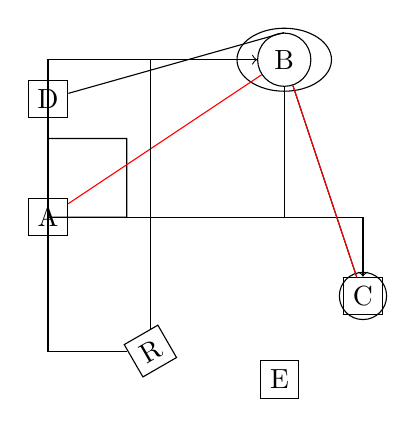
\begin{tikzpicture}[node distance=15mm]
  \node[draw] (a) at (0,0) {A};
  \node[draw,circle] (b) at (3,2) {B};
  \node[draw] (c) at (4,-1) {C};
  \draw[->] (a) |- (b);
  \draw[->] (a) -| (c);
  \draw (b) -- (c) -- cycle;
  \draw (c) circle (3mm) (b) ellipse (6mm and 4mm) (a) rectangle (1,1);
  \draw[red] (a) {-- (b)} -- (c);
  \node[draw,above of=a] (d) {D};
  \node[draw,below left of=c] {E};
  \draw (d) to (b.north);
  \node[draw,rotate=30] (r) at (1.3,-1.7) {R};
  \draw (r) |- (b) (b) |- (a) (r) -| (d);
\end{tikzpicture}
\end{center}
\end{document}
